\documentclass[../../../../doc.tex]{subfiles}

\begin{document}
\subsection{Algorytm A*}

Algorytm A* jest algorytmem wyszukiwania ścieżki w grafie, który znajduje najkrótszą ścieżkę między punktem startowym a docelowym. Wykorzystuje funkcję heurystyczną do optymalizacji procesu przeszukiwania.

\subsubsection{Opis działania algorytmu}

Algorytm łączy zalety przeszukiwania wszerz (BFS) i zachłannego przeszukiwania najlepszego pierwszego (Best-First Search). Działa poprzez minimalizację funkcji kosztu:
\[
  f(n) = g(n) + h(n)
\]
gdzie:
\begin{itemize}
  \item $g(n)$ - rzeczywisty koszt dotarcia z węzła startowego do bieżącego
  \item $h(n)$ - heurystyczny koszt dotarcia z bieżącego węzła do celu
\end{itemize}

\subsubsection{Inicjalizacja}
\begin{enumerate}
  \item Inicjalizacja struktur danych:
        \begin{itemize}
          \item \texttt{state} - mapa stanów węzłów (przechowuje $g(n)$ i poprzednika)
          \item \texttt{sortedQueue} - kolejka priorytetowa węzłów (posortowana po $f(n)$)
        \end{itemize}
  \item Dodanie węzła startowego:
        \begin{itemize}
          \item $g(\text{start}) = 0$
          \item $f(\text{start}) = h(\text{start})$
          \item Oznaczenie startu jako \texttt{queued}
        \end{itemize}
\end{enumerate}

\subsubsection{Funkcja heurystyczna}
Wykorzystana heurystyka to \textbf{odległość Manhattan (Taxicab)}:
\[
  h(n) = |n_x - \text{end}_x| + |n_y - \text{end}_y|
\]
Zapewnia dopuszczalność (nie przeszacowuje kosztu).

\subsubsection{Główna pętla algorytmu}
\begin{algorithmic}
  \WHILE{kolejka nie jest pusta}
  \STATE Pobierz węzeł o minimalnym $f(n)$ z \texttt{sortedQueue}
  \STATE Oznacz bieżący węzeł jako \texttt{candidate}
  \IF{bieżący węzeł jest metą}
  \STATE Przerwij pętlę
  \ENDIF
  \FOR{każdego sąsiada}
  \IF{sąsiad nie jest kolizją i nie był odwiedzony}
  \STATE $g_{\text{new}} \gets g(\text{current}) + 1$
  \STATE $f_{\text{new}} \gets g_{\text{new}} + h(\text{sąsiad})$
  \STATE Zapisz stan: $g = g_{\text{new}}$, poprzednik = currentNodePos
  \STATE Wstaw do kolejki z priorytetem $f_{\text{new}}$
  \STATE Oznacz jako \texttt{queued}
  \ENDIF
  \ENDFOR
  \ENDWHILE
\end{algorithmic}

\subsubsection{Budowanie ścieżki}
\begin{enumerate}
  \item \textbf{Śledzenie wsteczne:}
        \begin{itemize}
          \item Rozpocznij od mety
          \item Podążaj do poprzedników aż do startu
          \item Oznaczaj węzły jako \texttt{selected}
        \end{itemize}
  \item \textbf{Końcowe przetwarzanie:}
        \begin{itemize}
          \item Odwróć ścieżkę (start $\rightarrow$ meta)
          \item Oznacz start jako \texttt{selected}
        \end{itemize}
\end{enumerate}


\subsubsection{Złożoność obliczeniowa}
\begin{itemize}
  \item \textbf{Czasowa}: $O(n^2)$ (dla implementacji z listą)
  \item \textbf{Pamięciowa}: $O(n)$ (przechowywanie stanów i kolejki)
\end{itemize}
Przykład działania algorytmu przedstawia \cref{fig:astar_solve_steps}.

\begin{multicols}{2}
  \begin{figure}[H]
\centering
\begin{minipage}[t]{0.48\textwidth}
\centering
          
  \begin{tikzpicture}[scale=0.8]
  \node at (1.5, 0.5){\color{blue}\faIcon{user}};
\fill[gray] (2, 0) rectangle (3, 1);
\fill[gray] (0, 1) rectangle (1, 2);
\fill[gray] (2, 1) rectangle (3, 2);
\fill[gray] (4, 1) rectangle (5, 2);
\fill[gray] (0, 2) rectangle (1, 3);
\fill[gray] (2, 2) rectangle (3, 3);
\fill[gray] (4, 2) rectangle (5, 3);
\node at (4.5, 3.5){\color{blue}\faIcon{home}};
\fill[gray] (0, 4) rectangle (1, 5);
\fill[gray] (1, 4) rectangle (2, 5);
\fill[gray] (3, 4) rectangle (4, 5);
\fill[gray] (4, 4) rectangle (5, 5);
\draw[black] grid (5, 5);
  \end{tikzpicture}
  
          \caption{\centering Dodaj do kolejki węzeł (1,0).}
          \label{fig:astar_solve_steps_start}
\end{minipage}\hfill
\begin{minipage}[t]{0.48\textwidth}
          \centering
          
  \begin{tikzpicture}[scale=0.8]
  \node at (1.5, 0.5){\color{blue}\faIcon{user}};
\fill[gray] (2, 0) rectangle (3, 1);
\fill[gray] (0, 1) rectangle (1, 2);
\fill[gray] (2, 1) rectangle (3, 2);
\fill[gray] (4, 1) rectangle (5, 2);
\fill[gray] (0, 2) rectangle (1, 3);
\fill[gray] (2, 2) rectangle (3, 3);
\fill[gray] (4, 2) rectangle (5, 3);
\node at (4.5, 3.5){\color{blue}\faIcon{home}};
\fill[gray] (0, 4) rectangle (1, 5);
\fill[gray] (1, 4) rectangle (2, 5);
\fill[gray] (3, 4) rectangle (4, 5);
\fill[gray] (4, 4) rectangle (5, 5);
\draw[black] grid (5, 5);
  \end{tikzpicture}
  
          \caption{\centering Rozpatrz pole (1,0).}
\end{minipage}
\end{figure}

\begin{figure}[H]
\centering
\begin{minipage}[t]{0.48\textwidth}
          \centering
          
  \begin{tikzpicture}[scale=0.8]
  \node at (1.5, 0.5){\color{blue}\faIcon{user}};
\fill[gray] (2, 0) rectangle (3, 1);
\fill[gray] (0, 1) rectangle (1, 2);
\node at (1.5, 1.5){\color{purple}\faIcon{hourglass}};
\fill[gray] (2, 1) rectangle (3, 2);
\fill[gray] (4, 1) rectangle (5, 2);
\fill[gray] (0, 2) rectangle (1, 3);
\fill[gray] (2, 2) rectangle (3, 3);
\fill[gray] (4, 2) rectangle (5, 3);
\node at (4.5, 3.5){\color{blue}\faIcon{home}};
\fill[gray] (0, 4) rectangle (1, 5);
\fill[gray] (1, 4) rectangle (2, 5);
\fill[gray] (3, 4) rectangle (4, 5);
\fill[gray] (4, 4) rectangle (5, 5);
\draw[black] grid (5, 5);
  \end{tikzpicture}
  
          \caption{\centering Dodaj do kolejki węzeł (1,1).}
\end{minipage}\hfill
\begin{minipage}[t]{0.48\textwidth}
          \centering
          
  \begin{tikzpicture}[scale=0.8]
  \node at (0.5, 0.5){\color{purple}\faIcon{hourglass}};
\node at (1.5, 0.5){\color{blue}\faIcon{user}};
\fill[gray] (2, 0) rectangle (3, 1);
\fill[gray] (0, 1) rectangle (1, 2);
\node at (1.5, 1.5){\color{purple}\faIcon{hourglass}};
\fill[gray] (2, 1) rectangle (3, 2);
\fill[gray] (4, 1) rectangle (5, 2);
\fill[gray] (0, 2) rectangle (1, 3);
\fill[gray] (2, 2) rectangle (3, 3);
\fill[gray] (4, 2) rectangle (5, 3);
\node at (4.5, 3.5){\color{blue}\faIcon{home}};
\fill[gray] (0, 4) rectangle (1, 5);
\fill[gray] (1, 4) rectangle (2, 5);
\fill[gray] (3, 4) rectangle (4, 5);
\fill[gray] (4, 4) rectangle (5, 5);
\draw[black] grid (5, 5);
  \end{tikzpicture}
  
          \caption{\centering Dodaj do kolejki węzeł (0,0).}
\end{minipage}
\end{figure}

\begin{figure}[H]
\centering
\begin{minipage}[t]{0.48\textwidth}
          \centering
          
  \begin{tikzpicture}[scale=0.8]
  \node at (0.5, 0.5){\color{purple}\faIcon{hourglass}};
\node at (1.5, 0.5){\color{blue}\faIcon{user}};
\fill[gray] (2, 0) rectangle (3, 1);
\fill[gray] (0, 1) rectangle (1, 2);
\node at (1.5, 1.5){\color{orange}\faIcon{arrows-alt}};
\fill[gray] (2, 1) rectangle (3, 2);
\fill[gray] (4, 1) rectangle (5, 2);
\fill[gray] (0, 2) rectangle (1, 3);
\fill[gray] (2, 2) rectangle (3, 3);
\fill[gray] (4, 2) rectangle (5, 3);
\node at (4.5, 3.5){\color{blue}\faIcon{home}};
\fill[gray] (0, 4) rectangle (1, 5);
\fill[gray] (1, 4) rectangle (2, 5);
\fill[gray] (3, 4) rectangle (4, 5);
\fill[gray] (4, 4) rectangle (5, 5);
\draw[black] grid (5, 5);
  \end{tikzpicture}
  
          \caption{\centering Rozpatrz pole (1,1).}
\end{minipage}\hfill
\begin{minipage}[t]{0.48\textwidth}
          \centering
          
  \begin{tikzpicture}[scale=0.8]
  \node at (0.5, 0.5){\color{purple}\faIcon{hourglass}};
\node at (1.5, 0.5){\color{blue}\faIcon{user}};
\fill[gray] (2, 0) rectangle (3, 1);
\fill[gray] (0, 1) rectangle (1, 2);
\node at (1.5, 1.5){\color{orange}\faIcon{arrows-alt}};
\fill[gray] (2, 1) rectangle (3, 2);
\fill[gray] (4, 1) rectangle (5, 2);
\fill[gray] (0, 2) rectangle (1, 3);
\node at (1.5, 2.5){\color{purple}\faIcon{hourglass}};
\fill[gray] (2, 2) rectangle (3, 3);
\fill[gray] (4, 2) rectangle (5, 3);
\node at (4.5, 3.5){\color{blue}\faIcon{home}};
\fill[gray] (0, 4) rectangle (1, 5);
\fill[gray] (1, 4) rectangle (2, 5);
\fill[gray] (3, 4) rectangle (4, 5);
\fill[gray] (4, 4) rectangle (5, 5);
\draw[black] grid (5, 5);
  \end{tikzpicture}
  
          \caption{\centering Dodaj do kolejki węzeł (1,2).}
\end{minipage}
\end{figure}

\begin{figure}[H]
\centering
\begin{minipage}[t]{0.48\textwidth}
          \centering
          
  \begin{tikzpicture}[scale=0.8]
  \node at (0.5, 0.5){\color{purple}\faIcon{hourglass}};
\node at (1.5, 0.5){\color{blue}\faIcon{user}};
\fill[gray] (2, 0) rectangle (3, 1);
\fill[gray] (0, 1) rectangle (1, 2);
\node at (1.5, 1.5){\color{orange}\faIcon{arrows-alt}};
\fill[gray] (2, 1) rectangle (3, 2);
\fill[gray] (4, 1) rectangle (5, 2);
\fill[gray] (0, 2) rectangle (1, 3);
\node at (1.5, 2.5){\color{orange}\faIcon{arrows-alt}};
\fill[gray] (2, 2) rectangle (3, 3);
\fill[gray] (4, 2) rectangle (5, 3);
\node at (4.5, 3.5){\color{blue}\faIcon{home}};
\fill[gray] (0, 4) rectangle (1, 5);
\fill[gray] (1, 4) rectangle (2, 5);
\fill[gray] (3, 4) rectangle (4, 5);
\fill[gray] (4, 4) rectangle (5, 5);
\draw[black] grid (5, 5);
  \end{tikzpicture}
  
          \caption{\centering Rozpatrz pole (1,2).}
\end{minipage}\hfill
\begin{minipage}[t]{0.48\textwidth}
          \centering
          
  \begin{tikzpicture}[scale=0.8]
  \node at (0.5, 0.5){\color{purple}\faIcon{hourglass}};
\node at (1.5, 0.5){\color{blue}\faIcon{user}};
\fill[gray] (2, 0) rectangle (3, 1);
\fill[gray] (0, 1) rectangle (1, 2);
\node at (1.5, 1.5){\color{orange}\faIcon{arrows-alt}};
\fill[gray] (2, 1) rectangle (3, 2);
\fill[gray] (4, 1) rectangle (5, 2);
\fill[gray] (0, 2) rectangle (1, 3);
\node at (1.5, 2.5){\color{orange}\faIcon{arrows-alt}};
\fill[gray] (2, 2) rectangle (3, 3);
\fill[gray] (4, 2) rectangle (5, 3);
\node at (1.5, 3.5){\color{purple}\faIcon{hourglass}};
\node at (4.5, 3.5){\color{blue}\faIcon{home}};
\fill[gray] (0, 4) rectangle (1, 5);
\fill[gray] (1, 4) rectangle (2, 5);
\fill[gray] (3, 4) rectangle (4, 5);
\fill[gray] (4, 4) rectangle (5, 5);
\draw[black] grid (5, 5);
  \end{tikzpicture}
  
          \caption{\centering Dodaj do kolejki węzeł (1,3).}
\end{minipage}
\end{figure}

\begin{figure}[H]
\centering
\begin{minipage}[t]{0.48\textwidth}
          \centering
          
  \begin{tikzpicture}[scale=0.8]
  \node at (0.5, 0.5){\color{purple}\faIcon{hourglass}};
\node at (1.5, 0.5){\color{blue}\faIcon{user}};
\fill[gray] (2, 0) rectangle (3, 1);
\fill[gray] (0, 1) rectangle (1, 2);
\node at (1.5, 1.5){\color{orange}\faIcon{arrows-alt}};
\fill[gray] (2, 1) rectangle (3, 2);
\fill[gray] (4, 1) rectangle (5, 2);
\fill[gray] (0, 2) rectangle (1, 3);
\node at (1.5, 2.5){\color{orange}\faIcon{arrows-alt}};
\fill[gray] (2, 2) rectangle (3, 3);
\fill[gray] (4, 2) rectangle (5, 3);
\node at (1.5, 3.5){\color{orange}\faIcon{arrows-alt}};
\node at (4.5, 3.5){\color{blue}\faIcon{home}};
\fill[gray] (0, 4) rectangle (1, 5);
\fill[gray] (1, 4) rectangle (2, 5);
\fill[gray] (3, 4) rectangle (4, 5);
\fill[gray] (4, 4) rectangle (5, 5);
\draw[black] grid (5, 5);
  \end{tikzpicture}
  
          \caption{\centering Rozpatrz pole (1,3).}
\end{minipage}\hfill
\begin{minipage}[t]{0.48\textwidth}
          \centering
          
  \begin{tikzpicture}[scale=0.8]
  \node at (0.5, 0.5){\color{purple}\faIcon{hourglass}};
\node at (1.5, 0.5){\color{blue}\faIcon{user}};
\fill[gray] (2, 0) rectangle (3, 1);
\fill[gray] (0, 1) rectangle (1, 2);
\node at (1.5, 1.5){\color{orange}\faIcon{arrows-alt}};
\fill[gray] (2, 1) rectangle (3, 2);
\fill[gray] (4, 1) rectangle (5, 2);
\fill[gray] (0, 2) rectangle (1, 3);
\node at (1.5, 2.5){\color{orange}\faIcon{arrows-alt}};
\fill[gray] (2, 2) rectangle (3, 3);
\fill[gray] (4, 2) rectangle (5, 3);
\node at (0.5, 3.5){\color{purple}\faIcon{hourglass}};
\node at (1.5, 3.5){\color{orange}\faIcon{arrows-alt}};
\node at (4.5, 3.5){\color{blue}\faIcon{home}};
\fill[gray] (0, 4) rectangle (1, 5);
\fill[gray] (1, 4) rectangle (2, 5);
\fill[gray] (3, 4) rectangle (4, 5);
\fill[gray] (4, 4) rectangle (5, 5);
\draw[black] grid (5, 5);
  \end{tikzpicture}
  
          \caption{\centering Dodaj do kolejki węzeł (0,3).}
\end{minipage}
\end{figure}

\begin{figure}[H]
\centering
\begin{minipage}[t]{0.48\textwidth}
          \centering
          
  \begin{tikzpicture}[scale=0.8]
  \node at (0.5, 0.5){\color{purple}\faIcon{hourglass}};
\node at (1.5, 0.5){\color{blue}\faIcon{user}};
\fill[gray] (2, 0) rectangle (3, 1);
\fill[gray] (0, 1) rectangle (1, 2);
\node at (1.5, 1.5){\color{orange}\faIcon{arrows-alt}};
\fill[gray] (2, 1) rectangle (3, 2);
\fill[gray] (4, 1) rectangle (5, 2);
\fill[gray] (0, 2) rectangle (1, 3);
\node at (1.5, 2.5){\color{orange}\faIcon{arrows-alt}};
\fill[gray] (2, 2) rectangle (3, 3);
\fill[gray] (4, 2) rectangle (5, 3);
\node at (0.5, 3.5){\color{purple}\faIcon{hourglass}};
\node at (1.5, 3.5){\color{orange}\faIcon{arrows-alt}};
\node at (2.5, 3.5){\color{purple}\faIcon{hourglass}};
\node at (4.5, 3.5){\color{blue}\faIcon{home}};
\fill[gray] (0, 4) rectangle (1, 5);
\fill[gray] (1, 4) rectangle (2, 5);
\fill[gray] (3, 4) rectangle (4, 5);
\fill[gray] (4, 4) rectangle (5, 5);
\draw[black] grid (5, 5);
  \end{tikzpicture}
  
          \caption{\centering Dodaj do kolejki węzeł (2,3).}
\end{minipage}\hfill
\begin{minipage}[t]{0.48\textwidth}
          \centering
          
  \begin{tikzpicture}[scale=0.8]
  \node at (0.5, 0.5){\color{purple}\faIcon{hourglass}};
\node at (1.5, 0.5){\color{blue}\faIcon{user}};
\fill[gray] (2, 0) rectangle (3, 1);
\fill[gray] (0, 1) rectangle (1, 2);
\node at (1.5, 1.5){\color{orange}\faIcon{arrows-alt}};
\fill[gray] (2, 1) rectangle (3, 2);
\fill[gray] (4, 1) rectangle (5, 2);
\fill[gray] (0, 2) rectangle (1, 3);
\node at (1.5, 2.5){\color{orange}\faIcon{arrows-alt}};
\fill[gray] (2, 2) rectangle (3, 3);
\fill[gray] (4, 2) rectangle (5, 3);
\node at (0.5, 3.5){\color{purple}\faIcon{hourglass}};
\node at (1.5, 3.5){\color{orange}\faIcon{arrows-alt}};
\node at (2.5, 3.5){\color{orange}\faIcon{arrows-alt}};
\node at (4.5, 3.5){\color{blue}\faIcon{home}};
\fill[gray] (0, 4) rectangle (1, 5);
\fill[gray] (1, 4) rectangle (2, 5);
\fill[gray] (3, 4) rectangle (4, 5);
\fill[gray] (4, 4) rectangle (5, 5);
\draw[black] grid (5, 5);
  \end{tikzpicture}
  
          \caption{\centering Rozpatrz pole (2,3).}
\end{minipage}
\end{figure}

\begin{figure}[H]
\centering
\begin{minipage}[t]{0.48\textwidth}
          \centering
          
  \begin{tikzpicture}[scale=0.8]
  \node at (0.5, 0.5){\color{purple}\faIcon{hourglass}};
\node at (1.5, 0.5){\color{blue}\faIcon{user}};
\fill[gray] (2, 0) rectangle (3, 1);
\fill[gray] (0, 1) rectangle (1, 2);
\node at (1.5, 1.5){\color{orange}\faIcon{arrows-alt}};
\fill[gray] (2, 1) rectangle (3, 2);
\fill[gray] (4, 1) rectangle (5, 2);
\fill[gray] (0, 2) rectangle (1, 3);
\node at (1.5, 2.5){\color{orange}\faIcon{arrows-alt}};
\fill[gray] (2, 2) rectangle (3, 3);
\fill[gray] (4, 2) rectangle (5, 3);
\node at (0.5, 3.5){\color{purple}\faIcon{hourglass}};
\node at (1.5, 3.5){\color{orange}\faIcon{arrows-alt}};
\node at (2.5, 3.5){\color{orange}\faIcon{arrows-alt}};
\node at (4.5, 3.5){\color{blue}\faIcon{home}};
\fill[gray] (0, 4) rectangle (1, 5);
\fill[gray] (1, 4) rectangle (2, 5);
\node at (2.5, 4.5){\color{purple}\faIcon{hourglass}};
\fill[gray] (3, 4) rectangle (4, 5);
\fill[gray] (4, 4) rectangle (5, 5);
\draw[black] grid (5, 5);
  \end{tikzpicture}
  
          \caption{\centering Dodaj do kolejki węzeł (2,4).}
\end{minipage}\hfill
\begin{minipage}[t]{0.48\textwidth}
          \centering
          
  \begin{tikzpicture}[scale=0.8]
  \node at (0.5, 0.5){\color{purple}\faIcon{hourglass}};
\node at (1.5, 0.5){\color{blue}\faIcon{user}};
\fill[gray] (2, 0) rectangle (3, 1);
\fill[gray] (0, 1) rectangle (1, 2);
\node at (1.5, 1.5){\color{orange}\faIcon{arrows-alt}};
\fill[gray] (2, 1) rectangle (3, 2);
\fill[gray] (4, 1) rectangle (5, 2);
\fill[gray] (0, 2) rectangle (1, 3);
\node at (1.5, 2.5){\color{orange}\faIcon{arrows-alt}};
\fill[gray] (2, 2) rectangle (3, 3);
\fill[gray] (4, 2) rectangle (5, 3);
\node at (0.5, 3.5){\color{purple}\faIcon{hourglass}};
\node at (1.5, 3.5){\color{orange}\faIcon{arrows-alt}};
\node at (2.5, 3.5){\color{orange}\faIcon{arrows-alt}};
\node at (3.5, 3.5){\color{purple}\faIcon{hourglass}};
\node at (4.5, 3.5){\color{blue}\faIcon{home}};
\fill[gray] (0, 4) rectangle (1, 5);
\fill[gray] (1, 4) rectangle (2, 5);
\node at (2.5, 4.5){\color{purple}\faIcon{hourglass}};
\fill[gray] (3, 4) rectangle (4, 5);
\fill[gray] (4, 4) rectangle (5, 5);
\draw[black] grid (5, 5);
  \end{tikzpicture}
  
          \caption{\centering Dodaj do kolejki węzeł (3,3).}
\end{minipage}
\end{figure}

\begin{figure}[H]
\centering
\begin{minipage}[t]{0.48\textwidth}
          \centering
          
  \begin{tikzpicture}[scale=0.8]
  \node at (0.5, 0.5){\color{purple}\faIcon{hourglass}};
\node at (1.5, 0.5){\color{blue}\faIcon{user}};
\fill[gray] (2, 0) rectangle (3, 1);
\fill[gray] (0, 1) rectangle (1, 2);
\node at (1.5, 1.5){\color{orange}\faIcon{arrows-alt}};
\fill[gray] (2, 1) rectangle (3, 2);
\fill[gray] (4, 1) rectangle (5, 2);
\fill[gray] (0, 2) rectangle (1, 3);
\node at (1.5, 2.5){\color{orange}\faIcon{arrows-alt}};
\fill[gray] (2, 2) rectangle (3, 3);
\fill[gray] (4, 2) rectangle (5, 3);
\node at (0.5, 3.5){\color{purple}\faIcon{hourglass}};
\node at (1.5, 3.5){\color{orange}\faIcon{arrows-alt}};
\node at (2.5, 3.5){\color{orange}\faIcon{arrows-alt}};
\node at (3.5, 3.5){\color{orange}\faIcon{arrows-alt}};
\node at (4.5, 3.5){\color{blue}\faIcon{home}};
\fill[gray] (0, 4) rectangle (1, 5);
\fill[gray] (1, 4) rectangle (2, 5);
\node at (2.5, 4.5){\color{purple}\faIcon{hourglass}};
\fill[gray] (3, 4) rectangle (4, 5);
\fill[gray] (4, 4) rectangle (5, 5);
\draw[black] grid (5, 5);
  \end{tikzpicture}
  
          \caption{\centering Rozpatrz pole (3,3).}
\end{minipage}\hfill
\begin{minipage}[t]{0.48\textwidth}
          \centering
          
  \begin{tikzpicture}[scale=0.8]
  \node at (0.5, 0.5){\color{purple}\faIcon{hourglass}};
\node at (1.5, 0.5){\color{blue}\faIcon{user}};
\fill[gray] (2, 0) rectangle (3, 1);
\fill[gray] (0, 1) rectangle (1, 2);
\node at (1.5, 1.5){\color{orange}\faIcon{arrows-alt}};
\fill[gray] (2, 1) rectangle (3, 2);
\fill[gray] (4, 1) rectangle (5, 2);
\fill[gray] (0, 2) rectangle (1, 3);
\node at (1.5, 2.5){\color{orange}\faIcon{arrows-alt}};
\fill[gray] (2, 2) rectangle (3, 3);
\node at (3.5, 2.5){\color{purple}\faIcon{hourglass}};
\fill[gray] (4, 2) rectangle (5, 3);
\node at (0.5, 3.5){\color{purple}\faIcon{hourglass}};
\node at (1.5, 3.5){\color{orange}\faIcon{arrows-alt}};
\node at (2.5, 3.5){\color{orange}\faIcon{arrows-alt}};
\node at (3.5, 3.5){\color{orange}\faIcon{arrows-alt}};
\node at (4.5, 3.5){\color{blue}\faIcon{home}};
\fill[gray] (0, 4) rectangle (1, 5);
\fill[gray] (1, 4) rectangle (2, 5);
\node at (2.5, 4.5){\color{purple}\faIcon{hourglass}};
\fill[gray] (3, 4) rectangle (4, 5);
\fill[gray] (4, 4) rectangle (5, 5);
\draw[black] grid (5, 5);
  \end{tikzpicture}
  
          \caption{\centering Dodaj do kolejki węzeł (3,2).}
\end{minipage}
\end{figure}

\begin{figure}[H]
\centering
\begin{minipage}[t]{0.48\textwidth}
          \centering
          
  \begin{tikzpicture}[scale=0.8]
  \node at (0.5, 0.5){\color{purple}\faIcon{hourglass}};
\node at (1.5, 0.5){\color{blue}\faIcon{user}};
\fill[gray] (2, 0) rectangle (3, 1);
\fill[gray] (0, 1) rectangle (1, 2);
\node at (1.5, 1.5){\color{orange}\faIcon{arrows-alt}};
\fill[gray] (2, 1) rectangle (3, 2);
\fill[gray] (4, 1) rectangle (5, 2);
\fill[gray] (0, 2) rectangle (1, 3);
\node at (1.5, 2.5){\color{orange}\faIcon{arrows-alt}};
\fill[gray] (2, 2) rectangle (3, 3);
\node at (3.5, 2.5){\color{purple}\faIcon{hourglass}};
\fill[gray] (4, 2) rectangle (5, 3);
\node at (0.5, 3.5){\color{purple}\faIcon{hourglass}};
\node at (1.5, 3.5){\color{orange}\faIcon{arrows-alt}};
\node at (2.5, 3.5){\color{orange}\faIcon{arrows-alt}};
\node at (3.5, 3.5){\color{orange}\faIcon{arrows-alt}};
\node at (4.5, 3.5){\color{blue}\faIcon{home}};
\fill[gray] (0, 4) rectangle (1, 5);
\fill[gray] (1, 4) rectangle (2, 5);
\node at (2.5, 4.5){\color{purple}\faIcon{hourglass}};
\fill[gray] (3, 4) rectangle (4, 5);
\fill[gray] (4, 4) rectangle (5, 5);
\draw[black] grid (5, 5);
  \end{tikzpicture}
  
          \caption{\centering Dodaj do kolejki węzeł (4,3).}
\end{minipage}\hfill
\begin{minipage}[t]{0.48\textwidth}
          \centering
          
  \begin{tikzpicture}[scale=0.8]
  \node at (0.5, 0.5){\color{purple}\faIcon{hourglass}};
\node at (1.5, 0.5){\color{blue}\faIcon{user}};
\fill[gray] (2, 0) rectangle (3, 1);
\fill[gray] (0, 1) rectangle (1, 2);
\node at (1.5, 1.5){\color{orange}\faIcon{arrows-alt}};
\fill[gray] (2, 1) rectangle (3, 2);
\fill[gray] (4, 1) rectangle (5, 2);
\fill[gray] (0, 2) rectangle (1, 3);
\node at (1.5, 2.5){\color{orange}\faIcon{arrows-alt}};
\fill[gray] (2, 2) rectangle (3, 3);
\node at (3.5, 2.5){\color{purple}\faIcon{hourglass}};
\fill[gray] (4, 2) rectangle (5, 3);
\node at (0.5, 3.5){\color{purple}\faIcon{hourglass}};
\node at (1.5, 3.5){\color{orange}\faIcon{arrows-alt}};
\node at (2.5, 3.5){\color{orange}\faIcon{arrows-alt}};
\node at (3.5, 3.5){\color{orange}\faIcon{arrows-alt}};
\node at (4.5, 3.5){\color{blue}\faIcon{home}};
\fill[gray] (0, 4) rectangle (1, 5);
\fill[gray] (1, 4) rectangle (2, 5);
\node at (2.5, 4.5){\color{purple}\faIcon{hourglass}};
\fill[gray] (3, 4) rectangle (4, 5);
\fill[gray] (4, 4) rectangle (5, 5);
\draw[black] grid (5, 5);
  \end{tikzpicture}
  
          \caption{\centering Rozpatrz pole (4,3).}
\end{minipage}
\end{figure}

\begin{figure}[H]
\centering
\begin{minipage}[t]{0.48\textwidth}
          \centering
          
  \begin{tikzpicture}[scale=0.8]
  \node at (0.5, 0.5){\color{purple}\faIcon{hourglass}};
\node at (1.5, 0.5){\color{blue}\faIcon{user}};
\fill[gray] (2, 0) rectangle (3, 1);
\fill[gray] (0, 1) rectangle (1, 2);
\node at (1.5, 1.5){\color{orange}\faIcon{arrows-alt}};
\fill[gray] (2, 1) rectangle (3, 2);
\fill[gray] (4, 1) rectangle (5, 2);
\fill[gray] (0, 2) rectangle (1, 3);
\node at (1.5, 2.5){\color{orange}\faIcon{arrows-alt}};
\fill[gray] (2, 2) rectangle (3, 3);
\node at (3.5, 2.5){\color{purple}\faIcon{hourglass}};
\fill[gray] (4, 2) rectangle (5, 3);
\node at (0.5, 3.5){\color{purple}\faIcon{hourglass}};
\node at (1.5, 3.5){\color{orange}\faIcon{arrows-alt}};
\node at (2.5, 3.5){\color{orange}\faIcon{arrows-alt}};
\node at (3.5, 3.5){\color{orange}\faIcon{arrows-alt}};
\node at (4.5, 3.5){\color{blue}\faIcon{home}};
\fill[gray] (0, 4) rectangle (1, 5);
\fill[gray] (1, 4) rectangle (2, 5);
\node at (2.5, 4.5){\color{purple}\faIcon{hourglass}};
\fill[gray] (3, 4) rectangle (4, 5);
\fill[gray] (4, 4) rectangle (5, 5);
\draw[black] grid (5, 5);
  \end{tikzpicture}
  
          \caption{\centering Wybierz (4,3) do finalnej ścieżki.}
\end{minipage}\hfill
\begin{minipage}[t]{0.48\textwidth}
          \centering
          
  \begin{tikzpicture}[scale=0.8]
  \node at (0.5, 0.5){\color{purple}\faIcon{hourglass}};
\node at (1.5, 0.5){\color{blue}\faIcon{user}};
\fill[gray] (2, 0) rectangle (3, 1);
\fill[gray] (0, 1) rectangle (1, 2);
\node at (1.5, 1.5){\color{orange}\faIcon{arrows-alt}};
\fill[gray] (2, 1) rectangle (3, 2);
\fill[gray] (4, 1) rectangle (5, 2);
\fill[gray] (0, 2) rectangle (1, 3);
\node at (1.5, 2.5){\color{orange}\faIcon{arrows-alt}};
\fill[gray] (2, 2) rectangle (3, 3);
\node at (3.5, 2.5){\color{purple}\faIcon{hourglass}};
\fill[gray] (4, 2) rectangle (5, 3);
\node at (0.5, 3.5){\color{purple}\faIcon{hourglass}};
\node at (1.5, 3.5){\color{orange}\faIcon{arrows-alt}};
\node at (2.5, 3.5){\color{orange}\faIcon{arrows-alt}};
\node at (3.5, 3.5){\color{green}\faIcon{check}};
\node at (4.5, 3.5){\color{blue}\faIcon{home}};
\fill[gray] (0, 4) rectangle (1, 5);
\fill[gray] (1, 4) rectangle (2, 5);
\node at (2.5, 4.5){\color{purple}\faIcon{hourglass}};
\fill[gray] (3, 4) rectangle (4, 5);
\fill[gray] (4, 4) rectangle (5, 5);
\draw[black] grid (5, 5);
  \end{tikzpicture}
  
          \caption{\centering Wybierz (3,3) do finalnej ścieżki.}
\end{minipage}
\end{figure}

\begin{figure}[H]
\centering
\begin{minipage}[t]{0.48\textwidth}
          \centering
          
  \begin{tikzpicture}[scale=0.8]
  \node at (0.5, 0.5){\color{purple}\faIcon{hourglass}};
\node at (1.5, 0.5){\color{blue}\faIcon{user}};
\fill[gray] (2, 0) rectangle (3, 1);
\fill[gray] (0, 1) rectangle (1, 2);
\node at (1.5, 1.5){\color{orange}\faIcon{arrows-alt}};
\fill[gray] (2, 1) rectangle (3, 2);
\fill[gray] (4, 1) rectangle (5, 2);
\fill[gray] (0, 2) rectangle (1, 3);
\node at (1.5, 2.5){\color{orange}\faIcon{arrows-alt}};
\fill[gray] (2, 2) rectangle (3, 3);
\node at (3.5, 2.5){\color{purple}\faIcon{hourglass}};
\fill[gray] (4, 2) rectangle (5, 3);
\node at (0.5, 3.5){\color{purple}\faIcon{hourglass}};
\node at (1.5, 3.5){\color{orange}\faIcon{arrows-alt}};
\node at (2.5, 3.5){\color{green}\faIcon{check}};
\node at (3.5, 3.5){\color{green}\faIcon{check}};
\node at (4.5, 3.5){\color{blue}\faIcon{home}};
\fill[gray] (0, 4) rectangle (1, 5);
\fill[gray] (1, 4) rectangle (2, 5);
\node at (2.5, 4.5){\color{purple}\faIcon{hourglass}};
\fill[gray] (3, 4) rectangle (4, 5);
\fill[gray] (4, 4) rectangle (5, 5);
\draw[black] grid (5, 5);
  \end{tikzpicture}
  
          \caption{\centering Wybierz (2,3) do finalnej ścieżki.}
\end{minipage}\hfill
\begin{minipage}[t]{0.48\textwidth}
          \centering
          
  \begin{tikzpicture}[scale=0.8]
  \node at (0.5, 0.5){\color{purple}\faIcon{hourglass}};
\node at (1.5, 0.5){\color{blue}\faIcon{user}};
\fill[gray] (2, 0) rectangle (3, 1);
\fill[gray] (0, 1) rectangle (1, 2);
\node at (1.5, 1.5){\color{orange}\faIcon{arrows-alt}};
\fill[gray] (2, 1) rectangle (3, 2);
\fill[gray] (4, 1) rectangle (5, 2);
\fill[gray] (0, 2) rectangle (1, 3);
\node at (1.5, 2.5){\color{orange}\faIcon{arrows-alt}};
\fill[gray] (2, 2) rectangle (3, 3);
\node at (3.5, 2.5){\color{purple}\faIcon{hourglass}};
\fill[gray] (4, 2) rectangle (5, 3);
\node at (0.5, 3.5){\color{purple}\faIcon{hourglass}};
\node at (1.5, 3.5){\color{green}\faIcon{check}};
\node at (2.5, 3.5){\color{green}\faIcon{check}};
\node at (3.5, 3.5){\color{green}\faIcon{check}};
\node at (4.5, 3.5){\color{blue}\faIcon{home}};
\fill[gray] (0, 4) rectangle (1, 5);
\fill[gray] (1, 4) rectangle (2, 5);
\node at (2.5, 4.5){\color{purple}\faIcon{hourglass}};
\fill[gray] (3, 4) rectangle (4, 5);
\fill[gray] (4, 4) rectangle (5, 5);
\draw[black] grid (5, 5);
  \end{tikzpicture}
  
          \caption{\centering Wybierz (1,3) do finalnej ścieżki.}
\end{minipage}
\end{figure}

\begin{figure}[H]
\centering
\begin{minipage}[t]{0.48\textwidth}
          \centering
          
  \begin{tikzpicture}[scale=0.8]
  \node at (0.5, 0.5){\color{purple}\faIcon{hourglass}};
\node at (1.5, 0.5){\color{blue}\faIcon{user}};
\fill[gray] (2, 0) rectangle (3, 1);
\fill[gray] (0, 1) rectangle (1, 2);
\node at (1.5, 1.5){\color{orange}\faIcon{arrows-alt}};
\fill[gray] (2, 1) rectangle (3, 2);
\fill[gray] (4, 1) rectangle (5, 2);
\fill[gray] (0, 2) rectangle (1, 3);
\node at (1.5, 2.5){\color{green}\faIcon{check}};
\fill[gray] (2, 2) rectangle (3, 3);
\node at (3.5, 2.5){\color{purple}\faIcon{hourglass}};
\fill[gray] (4, 2) rectangle (5, 3);
\node at (0.5, 3.5){\color{purple}\faIcon{hourglass}};
\node at (1.5, 3.5){\color{green}\faIcon{check}};
\node at (2.5, 3.5){\color{green}\faIcon{check}};
\node at (3.5, 3.5){\color{green}\faIcon{check}};
\node at (4.5, 3.5){\color{blue}\faIcon{home}};
\fill[gray] (0, 4) rectangle (1, 5);
\fill[gray] (1, 4) rectangle (2, 5);
\node at (2.5, 4.5){\color{purple}\faIcon{hourglass}};
\fill[gray] (3, 4) rectangle (4, 5);
\fill[gray] (4, 4) rectangle (5, 5);
\draw[black] grid (5, 5);
  \end{tikzpicture}
  
          \caption{\centering Wybierz (1,2) do finalnej ścieżki.}
\end{minipage}\hfill
\begin{minipage}[t]{0.48\textwidth}
          \centering
          
  \begin{tikzpicture}[scale=0.8]
  \node at (0.5, 0.5){\color{purple}\faIcon{hourglass}};
\node at (1.5, 0.5){\color{blue}\faIcon{user}};
\fill[gray] (2, 0) rectangle (3, 1);
\fill[gray] (0, 1) rectangle (1, 2);
\node at (1.5, 1.5){\color{green}\faIcon{check}};
\fill[gray] (2, 1) rectangle (3, 2);
\fill[gray] (4, 1) rectangle (5, 2);
\fill[gray] (0, 2) rectangle (1, 3);
\node at (1.5, 2.5){\color{green}\faIcon{check}};
\fill[gray] (2, 2) rectangle (3, 3);
\node at (3.5, 2.5){\color{purple}\faIcon{hourglass}};
\fill[gray] (4, 2) rectangle (5, 3);
\node at (0.5, 3.5){\color{purple}\faIcon{hourglass}};
\node at (1.5, 3.5){\color{green}\faIcon{check}};
\node at (2.5, 3.5){\color{green}\faIcon{check}};
\node at (3.5, 3.5){\color{green}\faIcon{check}};
\node at (4.5, 3.5){\color{blue}\faIcon{home}};
\fill[gray] (0, 4) rectangle (1, 5);
\fill[gray] (1, 4) rectangle (2, 5);
\node at (2.5, 4.5){\color{purple}\faIcon{hourglass}};
\fill[gray] (3, 4) rectangle (4, 5);
\fill[gray] (4, 4) rectangle (5, 5);
\draw[black] grid (5, 5);
  \end{tikzpicture}
  
          \caption{\centering Wybierz (1,1) do finalnej ścieżki.}
\end{minipage}
\end{figure}

\begin{figure}[H]
\centering
\begin{minipage}[t]{0.48\textwidth}
          \centering
          
  \begin{tikzpicture}[scale=0.8]
  \node at (0.5, 0.5){\color{purple}\faIcon{hourglass}};
\node at (1.5, 0.5){\color{blue}\faIcon{user}};
\fill[gray] (2, 0) rectangle (3, 1);
\fill[gray] (0, 1) rectangle (1, 2);
\node at (1.5, 1.5){\color{green}\faIcon{check}};
\fill[gray] (2, 1) rectangle (3, 2);
\fill[gray] (4, 1) rectangle (5, 2);
\fill[gray] (0, 2) rectangle (1, 3);
\node at (1.5, 2.5){\color{green}\faIcon{check}};
\fill[gray] (2, 2) rectangle (3, 3);
\node at (3.5, 2.5){\color{purple}\faIcon{hourglass}};
\fill[gray] (4, 2) rectangle (5, 3);
\node at (0.5, 3.5){\color{purple}\faIcon{hourglass}};
\node at (1.5, 3.5){\color{green}\faIcon{check}};
\node at (2.5, 3.5){\color{green}\faIcon{check}};
\node at (3.5, 3.5){\color{green}\faIcon{check}};
\node at (4.5, 3.5){\color{blue}\faIcon{home}};
\fill[gray] (0, 4) rectangle (1, 5);
\fill[gray] (1, 4) rectangle (2, 5);
\node at (2.5, 4.5){\color{purple}\faIcon{hourglass}};
\fill[gray] (3, 4) rectangle (4, 5);
\fill[gray] (4, 4) rectangle (5, 5);
\draw[black] grid (5, 5);
  \end{tikzpicture}
  
          \caption{\centering Wybierz (1,0) do finalnej ścieżki.}
          \label{fig:astar_solve_steps_end}
\end{minipage}\hfill
\end{figure}

\end{multicols}

\end{document}
